\documentclass[spanish,a4paper,14pt,twoside]{report}

%%%%%%%%%%%%%%%%%%%%%%%%%%%%%%%%%%%%%%%%%%%%%%%%%%%%%%%%%%%%%%%%%%%%%%%%%%%%%%%
\usepackage[dvips]{graphicx}
\graphicspath{{images/}}

\usepackage[dvips]{epsfig}
%\usepackage[latin1]{inputenc}
\usepackage[utf8]{inputenc}
\usepackage[spanish]{babel}
\selectlanguage{spanish}
\usepackage{multirow} %tablas
\usepackage{float} % para usar [H]

\usepackage{hyperref}
%
\usepackage{listings}
\usepackage{color}

\lstloadlanguages{Ruby,HTML}
\lstset{
  language=Ruby,                      % C,Fortran,XML
  basicstyle=\small,             % Listados en small
  keywordstyle=\color{red},             % Palabras clave en rojo
  identifierstyle=\ttfamily,
  escapeinside={(*@}{@*)},
  commentstyle=\color{blue},            % comentarios en azul
  stringstyle=\color{green},            % cadenas en verde
  showstringspaces=false,
  frame=tb,
  captionpos=b,
  framextopmargin=2pt,
  framexbottommargin=2pt,
  framesep=0pt,
  belowskip=0pt,
  aboveskip=0pt,
  %belowcaptionskip=0pt,
  %abovecaptionskip=0pt,
  stepnumber=2,                                         % Opciones de lineas y etiquetas
  numberstyle=\small,
  numbersep=5pt,
  tabsize=1
}

%%
% Entornos para resumen y palabras clave en ingles y castellano
%%%%%%%%%%%%%%%%%%%%%%%%%%%%%%%%%%%%%%%%%%%%%%%%%%%%%%%%%%%%%%%%%%%%%%%%%%%%%%%
\newenvironment{summary}
{\par\noindent\begin{center}\textbf{Abstract}\end{center}\begin{itshape}\par\noindent}
{\end{itshape}}

\newenvironment{keywords}
{\begin{list}{}{\setlength{\leftmargin}{1em}}\item[\hskip\labelsep \bfseries Keywords:]}
{\end{list}}

\newenvironment{palabrasClave}
{\begin{list}{}{\setlength{\leftmargin}{1em}}\item[\hskip\labelsep \bfseries Palabras clave:]}
{\end{list}}
%%%%%%%%%%%%%%%%%%%%%%%%%%%%%%%%%%%%%%%%%%%%%%%%%%%%%%%%%%%%%%%%%%%%%%%%%%%%%%%

\begin{document}

%%%%%%%%%%%%%%%%%%%%%%%%%%%%%%%%%%%%%%%%%%%%%%%%%%%%%%%%%%%%%%%%%%%%%%%%%%%%%%%
% First Page: Title
%%%%%%%%%%%%%%%%%%%%%%%%%%%%%%%%%%%%%%%%%%%%%%%%%%%%%%%%%%%%%%%%%%%%%%%%%%%%%%%
\begin{titlepage}

  \begin{center}
    \vspace*{-1in}
    \begin{figure}[htb]
      \begin{center}
        
\includegraphics[width=8cm]{./images/logotipo-secundario-ULL-ESIT.jpg}
      \end{center}
    \end{figure}

    \begin{Large}
      \textbf{{\huge Trabajo Fin de Grado}}
    \end{Large}
    \rule{80mm}{0.3mm}\\
  \end{center}

  \begin{center}
    \vspace*{0.2in}
    \begin{LARGE}
      \textbf{Desarrollo en la nube: ChefManagement} \\
      Development in cloud: ChefManagement \\
    \end{LARGE}

    \vspace*{0.2in}
    \begin{large}
      ULL - ESIT\\
      {Aarón Socas Gaspar}\\
    \end{large}
    \vspace*{0.3in}
    \rule{80mm}{0.1mm}\\
    
    \vspace*{0.1in}
    \begin{large}
      Tutor \\
      Vicente Jose Blanco Perez \\
    \end{large}
    \vspace*{0.3in}
    \Large La Laguna, \today \\
  \end{center}

\end{titlepage}

%----------------------------------------------------------------------------

%    \pagestyle{empty}
%    \thispagestyle{empty}

%    \newcommand{\HRule}{\rule{\linewidth}{1mm}}
%    \setlength{\parindent}{0mm}
 %   \setlength{\parskip}{0mm}
 %   \vspace*{\stretch{1}}

 %   \begin{center}
 %   
\includegraphics[width=0.2\textwidth]{logotipo-secundario-ULL}\\[0.25cm]
 %   \end{center}

 %   \HRule
  %  \begin{flushright}
         %   {\Huge Acronimo} \\[2.5mm] 
         %   {\Huge Titulo en español} \\[2.5mm]
         %   {\Large \textit{Title in english}} \\[5mm]
         %   {\Large Aaron} \\[5mm]
         %   Dpto. de Ingeniería Informática y de Sistemas \\[5mm]
         %   Escuela Superior de Ingeniería y Tecnología \\[5mm]
            
         %   Trabajo de Fin de Grado \\
  %  \end{flushright}
  %  \HRule
  %  \vspace*{\stretch{2}}
  %  \begin{center}
 %     \Large La Laguna, \today 
 %   \end{center}

%    \setlength{\parindent}{5mm}


%%%%%%%%%%%%%%%%%%%%%%%%%%%%%%%%%%%%%%%%%%%%%%%%%%%%%%%%%%%%%%%%%%%%%%%%%%%%%%%
% Signature page (add the official stamp)
%%%%%%%%%%%%%%%%%%%%%%%%%%%%%%%%%%%%%%%%%%%%%%%%%%%%%%%%%%%%%%%%%%%%%%%%%%%%%%%
%\newpage
%\cleardoublepage
%\thispagestyle{empty}
\newpage{\pagestyle{empty}\cleardoublepage}
\pagenumbering{Roman} % para comenzar la numeracion de paginas en numeros romanos

D. \textbf{Vicente Jose Blanco Perez}, con N.I.F. 42.171.808-C profesor Titular de Universidad adscrito al Departamento de Ingeniería Informática y de Sistemas del Departamento de la Universidad de La Laguna, como tutor \\
\vspace*{0.6in}

\textbf{C E R T I F I C A} \\

\vspace*{0.1in}
Que la presente memoria titulada: \emph{Desarrollo en la nube: ChefManagement}. \\

\vspace*{0.1in}
ha sido realizada bajo su dirección por D. \textbf{Aarón Socas Gaspar}, con N.I.F. 78.702.938-C. \\

\vspace*{0.1in}
Y para que así conste, en cumplimiento de la legislación vigente y a los efectos portunos firman la presente en La Laguna a \today.   

%\cleardoublepage
%%%%%%%%%%%%%%%%%%%%%%%%%%%%%%%%%%%%%%%%%%%%%%%%%%%%%%%%%%%%%%%%%%%%%%%%%%%%%%%
%\thispagestyle{empty}
\newpage
{
\begin{flushright}
  \begin{LARGE}
    Agradecimientos
  \end{LARGE}
\end{flushright}

\hspace{3mm}

\begin{large}

Si he llegado hasta aquí ha sido gracias al apoyo de mi familia y mis amigos. Agradezco sus ánimos y ayuda por facilitar mi labor.

\vspace*{0.1in}
Una mención especial para mi madre Pilar, por enseñarme como persona lo que los libros no pueden,

\vspace*{0.1in}
a mi novia Pilar, por quererme, aguantarme y tener paciencia conmigo,

\vspace*{0.1in}
a mi hermano Josué, porque siempre está ahí y se preocupa por mí,

\vspace*{0.1in}
a mis tíos y abuelos, por ayudarme en todo y más,

\vspace*{0.1in}
a mi amigo Pablo, porque sé que puedo contar contigo para lo que sea.

\vspace*{0.1in}
También a mis profesores, que han sido muchas las horas en tutorías aguantando mis preguntas, en especial a Vicente Jose Blanco Perez, Casiano Rodríguez León, Gara Miranda Valladares y Jose Luis Roda García.

\hspace{3mm}

\end{large}

}

%%%%%%%%%%%%%%%%%%%%%%%%%%%%%%%%%%%%%%%%%%%%%%%%%%%%%%%%%%%%%%%%%%%%%%%%%%%%%%%
%LICENCIA
\newpage
{
\begin{center}
  \textbf{{\huge Licencia}}

  \vspace*{0.2in}
  \begin{figure}[htb]
    \begin{center}
      
\includegraphics[width=6cm]{./images/logotipo-licencia.png}
    \end{center}
  \end{figure}
  
  \vspace*{0.2in}
  \begin{Large}
    © Esta obra está bajo una licencia de Creative Commons Reconocimiento 4.0 Internacional.
  \end{Large}
\end{center}
}


%%%%%%%%%%%%%%%%%%%%%%%%%%%%%%%%%%%%%%%%%%%%%%%%%%%%%%%%%%%%%%%%%%%%%%%%%%%%%%%
%\cleardoublepage
\newpage
\begin{abstract}
{\em 
En este proyecto se abordarán aspectos del desarrollo de aplicaciones web y entornos de trabajo Cloud (PaaS). También el uso de la metodología ágil y el desarrollo dirigido por pruebas (TDD). La aplicación a desarrollar tiene como objetivo gestionar el escandallo de recetas haciendo uso de aplicaciones de terceros (APIs). Para hacer esto me ayudaré de herramientas orientadas al desarrollo de software, uso de repositorios (Github) y servidores de pruebas (Travis).
}

\vspace*{0.2in}
\begin{palabrasClave}
  Cloud, PaaS, TDD, escandallo, API.
\end{palabrasClave}

\end{abstract}
%%%%%%%%%%%%%%%%%%%%%%%%%%%%%%%%%%%%%%%%%%%%%%%%%%%%%%%%%%%%%%%%%%%%%%%%%%%%%%%

%%%%%%%%%%%%%%%%%%%%%%%%%%%%%%%%%%%%%%%%%%%%%%%%%%%%%%%%%%%%%%%%%%%%%%%%%%%%%%%
%\cleardoublepage
\newpage
\begin{summary}
{\em 
This project will approach issues web application development and Cloud working environment (PaaS). In addition to use of agile methodology and Test-driven development (TDD). The purpose of the application manage recipe cost production using third application (APIs). To do this, I will use tools oriented to software development, repository (Github) and test cloud (Travis).
}

\vspace*{0.2in}
\begin{keywords}
  Cloud, PaaS, TDD, recipe production cost, API.
\end{keywords}

\end{summary}
%%%%%%%%%%%%%%%%%%%%%%%%%%%%%%%%%%%%%%%%%%%%%%%%%%%%%%%%%%%%%%%%%%%%%%%%%%%%%%%

%%%%%%%%%%%%%%%%%%%%%%%%%%%%%%%%%%%%%%%%%%%%%%%%%%%%%%%%%%%%%%%%%%%%%%%%%%%%%%%
\newpage{\pagestyle{empty}\cleardoublepage}
\thispagestyle{empty}

%%%%%%%%%%%%%%%%%%%%%%%%%%%%%%%%%%%%%%%%%%%%%%%%%%%%%%%%%%%%%%%%%%%%%%%%%%%%%%%


\pagestyle{myheadings} %my head defined by markboth or markright
% No funciona bien \markboth sin "twoside" en \documentclass, pero al
% ponerlo se dan un montón de errores de underfull \vbox, con lo que no se
% ha puesto.
\markboth{Aarón Socas Gaspar}{Desarrollo en la nube: Chefmanagement}

%%%%%%%%%%%%%%%%%%%%%%%%%%%%%%%%%%%%%%%%%%%%%%%%%%%%%%%%%%%%%%%%%%%%%%%%%%%%%%%
%Numeracion en romanos
%\renewcommand{\thepage}{\roman{page}}
\renewcommand{\thepage}{\arabic{page}}
\setcounter{page}{1}

%%%%%%%%%%%%%%%%%%%%%%%%%%%%%%%%%%%%%%%%%%%%%%%%%%%%%%%%%%%%%%%%%%%%%%%%%%%%%%%

\tableofcontents

%%%%%%%%%%%%%%%%%%%%%%%%%%%%%%%%%%%%%%%%%%%%%%%%%%%%%%%%%%%%%%%%%%%%%%%%%%%%%%%
\newpage{\pagestyle{empty}\cleardoublepage}

\listoffigures

%%%%%%%%%%%%%%%%%%%%%%%%%%%%%%%%%%%%%%%%%%%%%%%%%%%%%%%%%%%%%%%%%%%%%%%%%%%%%%%
\newpage{\pagestyle{empty}\cleardoublepage}

\lstlistoflistings

%%%%%%%%%%%%%%%%%%%%%%%%%%%%%%%%%%%%%%%%%%%%%%%%%%%%%%%%%%%%%%%%%%%%%%%%%%%%%%%
\newpage{\pagestyle{empty}\cleardoublepage}

%%%%%%%%%%%%%%%%%%%%%%%%%%%%%%%%%%%%%%%%%%%%%%%%%%%%%%%%%%%%%%%%%%%%%%%%%%%%%%%
%Numeracion a partir del capitulo I
%\renewcommand{\thepage}{\arabic{page}}
%\setcounter{page}{1}

\chapter{Introducción}
\label{chapter:intro}

%\documentclass[a4paper,openright,14pt]{report}
%\usepackage[spanish]{babel}
%\selectlanguage{spanish}
%\usepackage[utf8]{inputenc}
%\usepackage{hyperref} %Para los enlaces
%\usepackage{multirow, array} % Para las tablas
%\usepackage{float}
%\usepackage{graphicx}

%%%%%%%%%%%%%%%%%%%%%%%%%%%%%%%%%%%%%%%%%%%%%%%%%%%%%%%%%%%%%%%%%%%%%%%%%%%%%
% Chapter 1: Introducción 
%%%%%%%%%%%%%%%%%%%%%%%%%%%%%%%%%%%%%%%%%%%%%%%%%%%%%%%%%%%%%%%%%%%%%%%%%%%%%%%

%---------------------------------------------------------------------------------
%\begin{document}
%\chapter{Introducción}\label{intro}

\section{Objetivos}\label{cap.1.1}
El objetivo de este trabajo de fin de grado (en adelante, TFG) es el desarrollo de una aplicación web para la gestión del escandallo, es decir, controlar el precio de producción de una receta. Para ello usaremos Cloud Servers, concretamente Google Cloud Platform, sin embargo, por algunas de las restricciones que mostraba, las cuales se describirán más adelante, se reorientó el TFG hacia otras plataformas como servicio (SaaS). Para su desarrollo usé la metodología de software ágil basada en el desarrollo dirigido por pruebas (TDD). Como framework, Sinatra (Ruby) para desarrollar la aplicación, integrar APIs de terceros, y hacer uso de varias nubes de producción a la vez y también herramientas de soporte para el desarrollo de software como son Github y Travis, entre otras.

\vspace*{0.2in}
\section{Antecedentes y estado actual del tema}\label{cap.1.2}
Los antecedentes y estudio de campo no sólo se centran en el tipo de aplicación que vamos a desarrollar, también tendremos en cuenta el entorno de producción, es decir, la nube donde estará disponible la aplicación web. Por lo tanto, tenemos dos puntos iniciales de estudio: 
\begin{itemize}
	\item Sobre la aplicación: 
	\begin{itemize}
		\item ¿Qué ofrece y por qué? 
		\item ¿Qué otras aplicaciones similares existen?
		\item Estudio del sector del mercado.
		\item Soporte y aspectos de la usabilidad.
	\end{itemize}

	\item Y respecto a la nube:
	\begin{itemize}
		\item ¿Cuál es la mejor nube que se adapte a nuestras necesidades?
		\item ¿Qué lenguajes y frameworks soporta?
		\item Período, costos, capacidad, etc.
	\end{itemize}
\end{itemize}

\vspace*{0.2in}
\begin{LARGE}
	\textbf {Aplicación}
\end{LARGE}

\vspace*{0.1in}
La finalidad de esta aplicación nace de la necesidad de optimizar los gastos, tanto en negocios de restauración como en los propios hogares. Hacer la comida controlando gastos es posible. En la actualidad existen en el mercado aplicaciones con esta idea, algunas de las mas destacadas son:
\begin{itemize}
	\item \href{https://recipecostcalculator.net/}{Recipe Cost Calculator}: Quizás sea la aplicación base como referencia, su fácil gestión y múltiples funciones la hace una herramienta útil y potente. Esta principalmente orientada a negocios.
	\item \href{http://www.recipe-costing.com/}{Recipe Costing}: Esta aplicación va más allá de las funcinalidades básicas, presenta extras como cálculos de menús, gestión de inventario, órdenes de compra a proveedores, etc.
	\item \href{http://developer.pearson.com/apis/pearson-kitchen-manager}{Pearson Kitchen Manager}: Se trata de una API, un banco de información que contiene más de 3000 mil recetas etiquetadas y con otra información como sus valores nutricionales.
	\item \href{https://itunes.apple.com/es/app/recipe-costing-calculator/id646877156?mt=8}{Recipe Costing Calculator}: Es más sencilla que las anteriores pero se trata de App disponible en iTunes. Las cosas más sencillas puden ser las más útiles, hay que tener en cuenta que un cocinero/a prefiere una tablet a un ordenador en la cocina.
\end{itemize}
La segmentación del mercado está orientado especialmente a negocios de restauración: comedores, restaurantes, bares, pastelerías, panaderías, etc. Por otro lado, existe otro sector que no se tiene tan en cuenta debido a que no genera tantos beneficios, se trata de los hogares. Las personas también pueden hacer uso de esta herramienta pues sus necesidades son las mismas pero a menor escala. En el próximo capítulo~\ref{chapter:dos}, se describe toda la funcionalidad de la aplicación, al igual que nos enseña como usarla y veremos las diferencias en la aplicación en función de a qué mercado está dirigido.\\

Por último, hay que tener en cuenta el soporte para la aplicación. Aprovechando la infraestructura y poder de Internet, la mejor opción es crear una aplicación web, que aunque en esta primera versión se diseñará de forma adaptativa, la idea es poder utilizarla en el futuro en dispositivos móviles y tablets. Además, se ha tenido en cuenta los aspectos de usabilidad durante su diseño.

\vspace*{0.3in}
\begin{LARGE}
	\textbf{{\huge Nube (cloud)}}
\end{LARGE}

\vspace*{0.1in}
Inicialmente la idea es trabajar en la \href{https://cloud.google.com/appengine/docs}{nube de Google}. Se trata de una plataforma como servicio (PaaS), la cual permite crear y mantener de forma sencilla una aplicación en la infraestructura de Google. Además permite una fácil escalabilidad de transeferencia de datos y almacenamiento gracias a sus módulos.\\

Empleando los conocimientos adquiridos durante los últimos cursos en Ruby y sus variedad de frameworks (Ruby on Rails, Padrino, Sinatra) lo usaré para crear la aplicación. Tras investigar y ver los servicios que ofrece Google App Engine (GAE) parece viable la puesta en marcha de la aplicación. GAE soporta cuatro lenguajes y sus correspondientes frameworks:
\begin{itemize}
	\item \href{https://cloud.google.com/appengine/docs/python/gettingstartedpython27/introduction}{Python} con webapp2 y Jinja2.
	\item \href{https://cloud.google.com/appengine/docs/java/gettingstarted/introduction}{Java} con maven.
	\item \href{https://cloud.google.com/appengine/docs/php/gettingstarted/introduction}{PHP} con Cloud SQL.
	\item \href{https://cloud.google.com/appengine/docs/go/gettingstarted/introduction}{Go} con el paquete html/plantilla. 
\end{itemize}

\begin{figure}[H]
	\centering
		
\includegraphics[width=10cm]{./images/lenguajes-GAE.png}
		\caption{Lenguajes soportados en GAE} \label{fig:lenguajes-GAE}
\end{figure}

Sin embargo, también es posible hacerlo funcionar en Ruby con la ayuda de java, juntos forman \href{http://jruby.org/}{Jruby}, el cual es una implementación 100\% del lenguaje Ruby. Además funciona como lenguaje embebido dentro de la máquina virtual de Java. Gracias a esta capa, podré programar en Ruby y Jruby establecerá una capa intermedia entre el código fuente en Ruby y el servidor en java. Para interactuar con la aplicación en la nube provee de una herramienta o kit, en este caso se trata de una gema llamada \href{https://rubygems.org/gems/google-appengine}{google-appengine}, sin embargo, la gema
dedicada a tal fin esta desfasada y el proyecto ha sido \href{https://code.google.com/p/appengine-jruby/}{archivado}.\\

Tras la incompatibilidad del proyecto de Jruby en GAE busco la opción más parecida posible que me ofrezca soporte, en este caso Google Cloud Platform. Tras investigar encuentro multitud de \href{https://cloud.google.com/launcher/explore}{lenguajes compatibles}, entre ellos Ruby, sin embargo, los servicios de esta nube son de pago y aunque existe una versión demo durante 60 días. Debido al tiempo que emplearía en el estudio, desarrollo y pruebas, este período puede resultar corto. Me pongo en contacto con el servicio de clientes y soporte de Google para bajar otras opciones, pero no ofrecen nada que me sea viable para desarrollar mi proyecto.\\

De esta forma se modifica el requisito inicial del TFG de usar los servicios de la nube de Google para encontrar y usar otros entornos de producción. La idea es intentar usar más de uno, demostrando la modularidad de la aplicación, esto significa que el código fuente de la aplicación debe ser único para las distintas nubes de producción. El siguiente paso es investigar las nubes que se ofertan. La siguiente tabla muestra un resumen:

\begin{table}[H]
	\centering
	\begin{tabular}{p{2cm} p{8cm}}
	\hline
	\textbf{Nube} & \textbf{Comentario} \\
	\hline \hline
	\href{https://cloud.google.com/free-trial/?hl=es&_ga=1.261030148.846668794.1427305506}{Google} & De pago. Prueba gratuita de 60 días. Multitud de servicios, distintos tipos de bbdd y soporta muchos \href{https://cloud.google.com/launcher/?hl=es}{lenguajes} y frameworks. \\
	\hline
	\href{http://azure.microsoft.com/en-us/}{Azure} & De pago. Prueba de 30 días. Soporta varios \href{https://tryappservice.azure.com/}{lenguajes}. \\
	\hline
	\href{https://c9.io/}{cloud9} & Se trata de un entorno de trabajo, una nube orientada al desarrollo, no es lo que buscamos. \\
	\hline
	\href{https://www.nitrous.io/}{nitrous} & Es similar a la anterior. Orientada al trabajo colaborativo en entornos de desarrollo. \\
	\hline
	\href{https://www.dotcloud.com/}{dotCloud} & Esta es una propuesta válida. Se trata de una nube de producción con servicios de pago y versión básica gratuita. Soporta varios \href{https://www.dotcloud.com/dev-center/guides}{lenguajes}. El uso de módulos como bbdd o rendimiento del servidor son de pago. \\
	\hline
	\href{https://www.heroku.com/}{Heroku} & Ideal para experimentar con aplicaciones en la nube en un módulo limitada. Su uso es ilimitado, pero tiene algunas \href{https://www.heroku.com/pricing}{condiciones}. Soporta varios \href{https://devcenter.heroku.com/categories/language-support}{lenguajes} y frameworks. \\
	\hline
	\href{https://www.openshift.com/}{OpenShift} & Es una alternativa muy interesante. Existe la opción de uso gratuito de hasta 3 aplicaciones. Soporta varios \href{https://www.openshift.com/promotions/try-openshift?sc_cid=70160000000UJArAAO&gclid=CMqo54DUy8cCFSMcwwodxLoGGQ}{lenguajes} y distintas versiones del mismo, así como 3 tipos de bbdd (PostgreSQL, MySQL y MongoDB) y los cartuchos (módulos) que añadamos son de pago. Podemos crear y subir nuestros propios cartuchos. \\
	\hline
	\href{https://www.appfog.com/}{appfog} & De pago con versión de prueba de 30 días. Soporta varios \href{https://www.ctl.io/appfog/}{lenguajes}. El enfoque de esta PaaS es facilitar el trabajo al equipo de desarrollo y que solo se centre en la aplicación y en los datos, mientras la nube gestionaría el resto. \\
	\hline
	\href{https://aws.amazon.com/es/?nc2=h_lg}{Amazon} & Presenta una gran infraestructura de servicios y recursos. Es de pago pero tiene una versión de prueba de 12 meses. Soporta varios lenguajes y dispone de multitud de productos orientados a distintos tipos de mercado. \\
	\hline
	\href{https://www.digitalocean.com/}{DigitalOcean} & Es de pago. Provee de infraestructura remota para que el desarrollador pueda lenvantor el tipo de servidor que desee. Soporta varios \href{https://www.digitalocean.com/community/}{lenguajes} y frameworks. \\
	\hline
	\href{http://www.cloud66.com/}{Cloud66} & Es de pago pero tiene un perídodo de 14 días de prueba. Esta orientada a mejora las aplicaciones que ya tenemos en otras nubes, en cuanto aspectos de crecimiento y seguridad. \\
	\hline
	\href{http://www.1and1.es/}{1 and 1} & Es de pago. Soporta diferentes lenguajes, frameworks y CMS. \\
	\hline
	\end{tabular}
	\caption{Production Clouds}
	\label{tabla:clouds}
\end{table}

Una vez analizadas se propone como entornos de producción las nubes Heroku y Openshift, de las cuales se entrará en detalle en el capítulo~\ref{chapter:tres}.

%----------------------------------------------------------------------------------

\vspace*{0.2in}
\section{Metodología de trabajo}\label{cap.1.3}

Durante la investigación y desarrollo de este proyecto se ha apostado por las metodologías ágiles, si bien no ha sido en un grupo de trabajo, se puede aplicar en lo que se refiere al análisis, al desarrollo y diseño de la aplicación y a las reuniones con el \emph{cliente}, cuyo rol lo asume el tutor junto con el de \emph{jefe de proyecto}. \\

Estos métodos están basados en el desarrollo iterativo e incremental, donde los requisitos y soluciones evolucionan mediante la colaboración de grupos. La idea es minimizar riesgos desarrollando software en períodos cortos. Este período se llama \textbf{iteración} cuya duración se define en función de los requisitos del proyecto, especialmente recursos de tiempo y humano. \\

\begin{figure}[H]
	\centering
	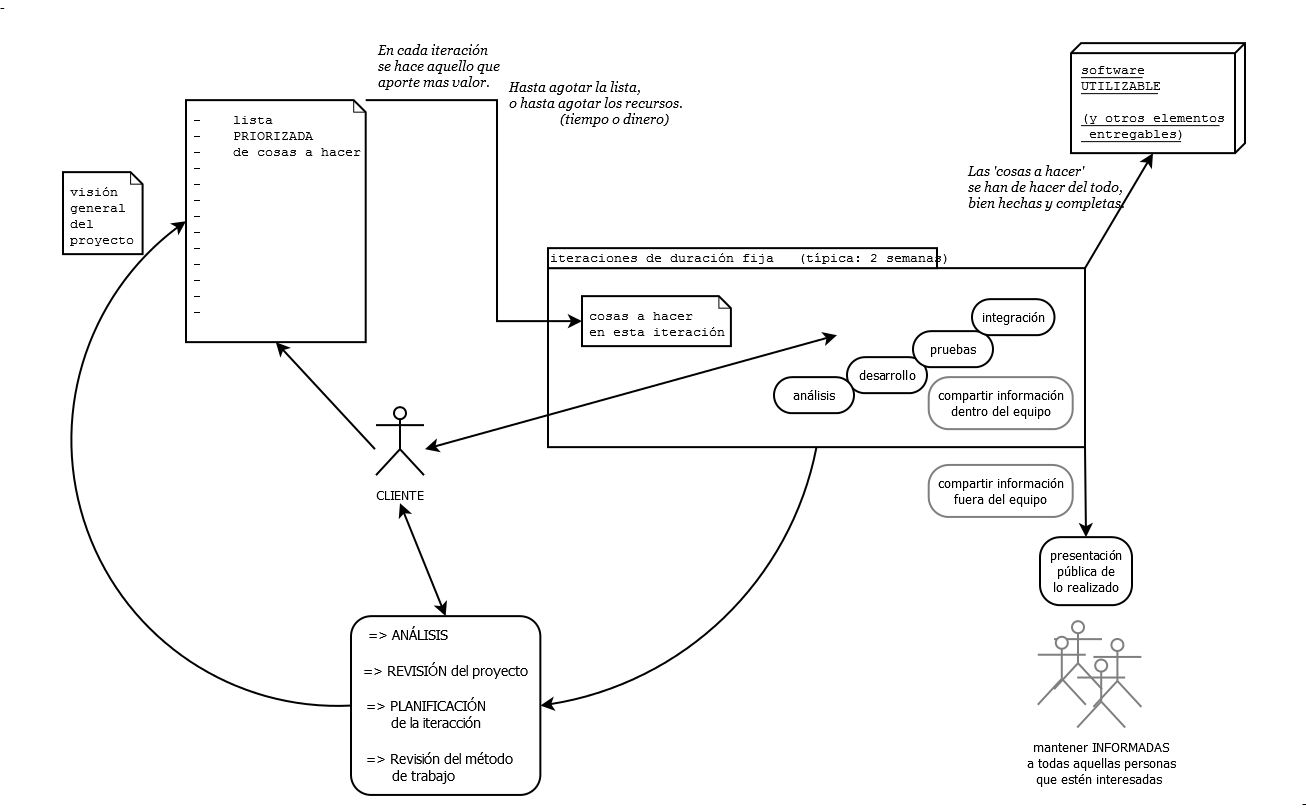
\includegraphics[width=14cm]{./images/metodologia-agil.png}
	\caption{Esquema de metodología ágil} \label{fig:metodologia}
\end{figure}

\vspace*{0.1in}
Cada iteración del ciclo de vida incluye:
\begin{itemize}
	\item Planificación: organización del trabajo durante una iteración. En este caso, la planificación corresponde con las tutorías y seguimiento semanal con el tutor.
	\item Análisis de requisitos: cada nueva funcionalidad o idea para la aplicación debe ser estudiada. Así, si por ejemplo, si quiero integrar una API debo considerar si es útil o no, si es compatible con los entornos de producción y con el lenguaje, documentarme para su integración en la aplicación, etc.
	\item Diseño: interfaz de la aplicación, características y aspectos de usabilidad.
	\item Codificación: corresponde por lo general a escribir código, aunque esto no se limita solo a realizar la propia aplicación, además se incluyen los tests y todos aquellos prototipos y pruebas durante la etapa de estudio de campo.
	\item Revisión: incluye superar los tests con éxito y la aceptación por parte del cliente.
	\item Documentación: para este trabajo en concreto, se realizó un diario semanal, cuya síntesis se engloba en este documento.
\end{itemize}

Durante este proyecto se ha seguido dicho ciclo de vida con especial importacia. He intentado adaptar la metodología Scrum a este trabajo, aunque no se ha tenido en cuenta  el aspecto de los roles. En Scrum se realizan entregas parciales y regulares del producto final. Scrum está especialmente indicado para proyectos en entornos complejos, donde se necesita obtener resultados pronto, donde los requisitos son cambiantes o poco definidos, donde la innovación, la competitividad, la flexibilidad y la productividad son fundamentales. \\

Cabe destacar dada la utilización del framework de Sintra, el uso inherente del modelo-vista-controlador (MVC) durante la etapa de diseño, desarrollo y pruebas. Se describirá detalladamente en el capítulo~\ref{chapter:cuatro} así como su uso para crear Chefmanagement.

%\end{document}


%---------------------------------------------------------------------------------
%Citando una entrada de memtfg.bib \cite{URL:GitHub}

%Incluyento una gráfica y referenciandola como Figura \ref{fig:prueba} y tambien un poco de código como Listado \ref{code:prueba}


%%%%%%%%%%%%%%%%%%%%%%%%%%%%%%%%%%%%%%%%%%%%%%%%%%%%%%%%%%%%%%%%%%%%%%%%%%%%%%%
\newpage{\pagestyle{empty}\cleardoublepage}
\thispagestyle{empty}

\chapter{Descripción de la aplicaci\'on}
\label{chapter:dos}

%%%%%%%%%%%%%%%%%%%%%%%%%%%%%%%%%%%%%%%%%%%%%%%%%%%%%%%%%%%%%%%%%%%%%%%%%%%%%%%
% Chapter 2: Descripción de la aplicación: ChefManagement
%%%%%%%%%%%%%%%%%%%%%%%%%%%%%%%%%%%%%%%%%%%%%%%%%%%%%%%%%%%%%%%%%%%%%%%%%%%%%%%

En el capítulo anterior~\ref{chapter:intro} se ha introducido tanto los antecedentes como se describió brevemente la aplicación. En este capítulo explicaremos toda las funcionalidades y sus características con detalle. \\

Partimos de qué tipo de aplicación queremos crear. Se trata de desarrollar un software que ayude a las personas a gestionar el costo de producción de las recetas, dependiendo del precio de sus ingredientes y el número de raciones. Ésta se llamará \textbf{ChefManagement} y sus características iniciales son:
\begin{itemize}
	\item Crear, ver, editar y eliminar recetas.
	\item Listar todas las recetas.
	\item Crear backup de las recetas y cargarlo si es necesario.
	\item Calcular el precio de una determinada receta para un determinado número de comensales.
\end{itemize}

Para esta primera versión, además de ser capaz de realizar esta serie de tareas, debe  cumplir con las necesidades y espectativas del usuario y facilitar su interacción con la aplicación. Éstos son sus requisitos iniciales:
\begin{itemize}
	\item Dos entornos de producción: la aplicación puede ser usada desde dos nubes diferentes.
	\item Tener en cuenta aspectos de usablidad: adaptación, entendimiento y facilidad de uso.
	\item Importar y exportar archivos en formato json: almacenar copias de las recetas en el equipo cliente y restaurarlas si es necesario.
	\item Accesso mediante registro o haciendo uso de APIs de distintas redes sociales como Google+ o Facebook. Hay que facilitar el acceso a los usuarios.
\end{itemize}

Tanto las características comos los requisitos de la aplicación serán aplicadas a la versión 1.0, pudiendo ser mejorados o añadidos más en futuras versiones~\ref{chapter:conclusiones}.

\vspace*{0.2in}
\section{Acceso a la aplicación}\label{cap.2.1}

Para usar esta aplicación podemos acceder directamente a sus entornos de producción:
\begin{itemize}
	\item \href{http://chefmanagement.herokuapp.com/}{Despliegue en Heroku}
	\item \href{http://chefmanagement-esit.rhcloud.com/}{Despliegue en OpenShift}
\end{itemize}

O bien acceder al \href{https://github.com/alu0100207385/ChefManagement}{repositorio} de la aplicación (se trata de licencia libre y código abierto) y seguir las instrucciones de instalación. \\

Una vez en la aplicación encontraremos una pantalla inicial de acceso, que nos permite acceder usando redes sociales, en este caso Google+ y Facebook. Esto es posible gracias al uso de su API (o interfaz de programación de aplicaciones) correspondiente, la cual es un conjunto de funciones o métodos que ofrece una librería para ser utilizado por otro software. En otras palabras, el equipo de desarrollo de Facebook crea esta herramienta para que otras aplicaciones, como Chefmanagement puedan hacer uso de ella. Esto tiene ventajas importantes como la seguridad, desde el punto de vista de desarrollo de software y la comodidad para los usuarios finales. \\

\begin{figure}[H]
	\centering
	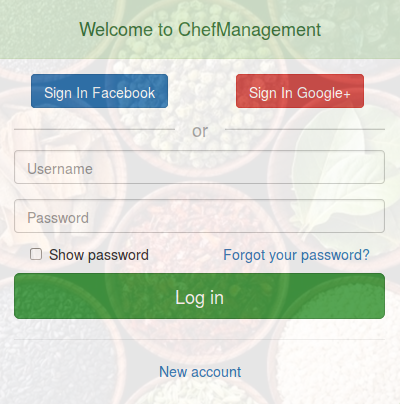
\includegraphics[width=8cm]{./images/chefmanagement-root.png}
	\caption{Acceso a la aplicación} \label{fig:chefmanagement-root}
\end{figure}

Además existe la opción de validarnos en la aplicación, una vez que se haya completado el registro. Si el usuario de entrada o contraseña fueran incorrectos la aplicación lo notificaría. En caso de pérdida de contraseña podemos solicitar una nueva accediendo al enlace \emph{Forgot your password?} y proporcionar nuestro nombre de usuario. Posteriormente puede modificarse la nueva contraseña en opciones~\ref{sec:cap.2.5}.

\begin{figure}[H]
	\centering
	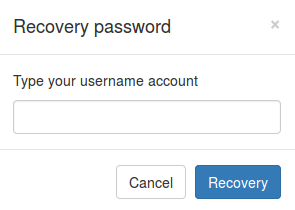
\includegraphics[width=8cm]{./images/chefmanagement-recovery.png}
	\caption{Recuperar contraseña} \label{fig:chefmanagement-recovery}
\end{figure}

Para registarse accedemos a través del enlace \emph{New account}. En caso de cualquier problema durante el proceso de registro, como que el correo o nombre de usuario estén en uso, la aplicación lo notificará al usuario.

\begin{figure}[H]
	\centering
	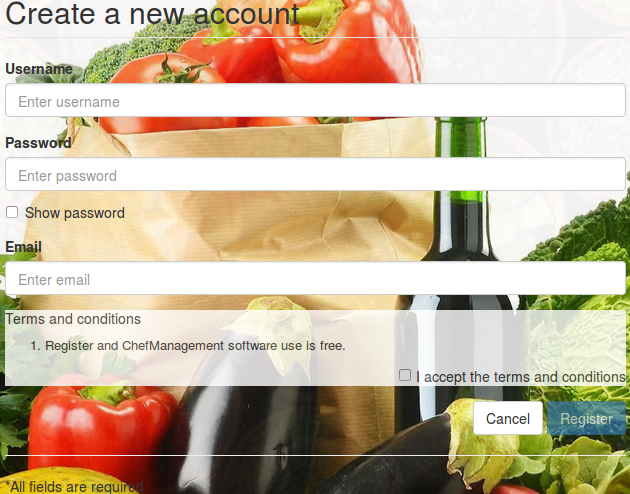
\includegraphics[width=8cm]{./images/chefmanagement-register.png}
	\caption{Registro} \label{fig:chefmanagement-register}
\end{figure}

Una vez dentro de la aplicación accederemos al \emph{home} del usuario. Existe un barra superior donde podemos acceder a la configuración y salir de la aplicación (Log out). También encontramos un menú lateral el cual facilita la interacción del usuario con la aplicación y ayudar a moverse y gestionar las distintas tareas. Por defecto, cuando accedemos a la aplicación, en \emph{home} se nos despliega la lista de recetas creadas por ese usuario. Las opciones del menú son las siguientes:

\begin{itemize}
	\item Recipe list: muestra el listado de recetas del usuario. Podemos acceder, editar y borrar recetas a través de esta lista.
	\item Recipe calculator: calcula el costo de producción de una receta y sus ingredientes para una determinada receta y raciones.
	\item New recipe: crea una nueva receta.
	\item Import: carga una copia de seguridad de las recetas del usuario.
	\item Export: almacena en el equipo local una copa de seguridad de las recetas del usuario.
\end{itemize}


\vspace*{0.2in}
\section{Crear recetas}\label{cap.2.2}

Para acceder a crear receta, nos situamos en el menú lateral y pinchamos en \textbf{New recipe}. Esto nos llevará a una nueva ventana, la cual presentará un formulario con una serie de campos que se detallan a continuación:

\begin{itemize}
	\item Name: es un campo obligatorio y clave primaria en la bbdd. Nombre de la receta.
	\item Rations: Numero de raciones para crear esa receta. Este campo es muy importante ya que se tomará como referencia para el cálculo de recetas dado un determinado número de platos.
	\item Cost: es un campo de lectura, se calcula acutomáticamente con cada ingrediente.
	\item Ration cost: relación entre el coste de la receta y el número de raciones.
	\item Order: campo que sirve como etiqueta. Indica si se trata de un primer o segundo plato, un postre, etc.
	\item Type: segundo campo de etiqueta. Nos da información sobre el tipo de comida: snack, comida casera y otros.
	\item Nivel: nivel de dificultad de producción de la receta.
	\item Time: horas y minutos que se estima que lleva preparar esa receta.
	\item Vegan: indica si la receta es apta para vegetarianos.
	\item Allergens: campo de texto para introducir alimentos que puedan producir alergias.
	\item Origin: información sobre el país originario de la receta.
\end{itemize}

Una vez completado podemos guardar la receta con el botón \textbf{Save recipe} o cancelar el proceso y volver a \emph{home}. Si guardamos la receta el sistema notificará de su registro en la bbdd y abrirá nuevos campos: 

\begin{itemize}
	\item Un área de texto desplegable que se utiliza para escribir las instrucciones de la receta. He utilizado la herramienta \href{http://ckeditor.com/}{ckeditor} para integrarla en la aplicación-
	\item Ingredientes, que puede ser:
		\begin{itemize}
			\item Un \textbf{nuevo ingrediente} creador por el usuario. Campos:
				\begin{itemize}
					\item Nombre del ingrediente
					\item Cantidad: puede ser: peso, volumen o una determinada unidad.
					\item Precio en relación con su cantidad
					\item El porcentaje de merma o pérdida del ingrediente durante su preparación.
				\end{itemize}
			\item \textbf{Una receta} ya creada por el usuario. De forma que las recetas puedan servir de base para crear otras, por ejemplo, la salsa de tomate es una receta que se puede usar en otras. Si una receta usa otra, la primera no puede ser usada para crear otra y no aparecerá como opción en este apartado.
		\end{itemize}
\end{itemize}

A medida que vayamos incluyendo ingredientes a la receta, en el margen lateral derecho se desplegará una lista informativa de la receta con los ingredientes agregados hasta el momento.

\vspace*{0.2in}
\section{Editar y eliminar recetas}\label{cap.2.3}

Desde el listado de recetas podemos editar o eliminar según nuestras necesidades. Para ello pinchamos en una determinada receta y accederemos a toda la información de la receta. Esta opción es de sólo lectura. En la parte superior derecha encontramos los iconos para eliminar y editar la receta. \\

Para eliminar la receta pulsamos el botón de eliminar. El programa pedirá la confirmación para eliminarla. Una vez eliminada no se puede recuperar. Las recetas que sirven de base a otras no pueden ser eliminadas hasta que no se rompa este vínculo, para ello debemos entrar en el modo edición. \\

Si pulsamos en edición, nos llevará a una nueva pantalla donde podemos editar todos los campos de la receta (excepto el nombre y los costos que se calculan automáticamente). Podemos añadir nuevos ingredientes, editar o borrar los actuales o bien borrar \emph{recetas base} (en futuras aplicaciones se recomienda poder añadir \emph{recetas bases}). Así mismo podemos editar las instrucciones de la receta. \\

\vspace*{0.2in}
\section{Calculadora}\label{cap.2.4}

Esta opción nos permite elegir entre el listado de recetas del usuario. Una vez hecho esto seleccionamos el número de raciones que queremos producir y pulsamos en calcular. Se mostrará una tabla resultante con el listado de ingredientes, sus cantidades para las raciones seleccionadas y su precio. De la misma forma se mostrarán las \emph{recetas bases} si contiene alguna y por último el precio de producción final. \\

A modo de información adicional se muestra las instrucciones de la \textbf{receta original}.

\vspace*{0.2in}
\section{Importar y exportar}\label{cap.2.5}

Estas opciones nos permiten crear y cargar una copia de seguridad de las recetas y sus ingredientes del usuario. Para crear una copia, seleccionamos la opción \textbf{Export} del menú lateral. Se mostrará un campo de texto para elegir el nombre del archivo, (por defecto \emph{recipe}) el cual podemos editar y pulsamos en crear. Se comprueba si la cadena introducida contiene caracteres inválidos, en caso contrario se notifica al usuario la operación exitosa y se descarga el archivo al equipo local en formato \textbf{json}. \\

Por otro lado, está la opción de cargar la copia de seguridad. Para ello pulsamos en la opción \textbf{Import}, nos permitirá seleccionar un archivo solo válido en formato json. Una vez seleccionado pulsamos en cargar, en caso de error, la aplicación lo notificará con un mensaje, y si el archivo se ha cargado correctamente nos redirige a \emph{home} con el listado de recetas. Hay que tener en cuenta que si cargamos una copia de seguridad borrará el contenido actual de recetas para cargar ésta.

\vspace*{0.2in}
\section{Opciones}\label{cap.2.5}

Las opciones se encuentran en la parte derecha de la barra superior de la aplicación. Si pulsamos nos lleva a una nueva pantalla que nos muestra el perfil del usuario. Éste se podrá editar en caso de que el usuario haya accedido mediante registro en la propia aplicación, si accedió vía redes sociales debe acceder a las mismas para editar su perfil. \\

También permite la opción de darse de baja de la aplicación. Ello conlleva el borrado de todas sus recetas de la bbdd.

\vspace*{0.2in}
\section{Diseño de la base de datos}\label{cap.2.6}

El modelo propuesto para esta primera versión atendiendo a los requisitos de la aplicación, es el siguiente:
\begin{itemize}
	\item \textbf{Usuarios (User):} Se trata del modelo base y del que depende la gestión del resto. Sus campos son: \emph{username}, \emph{email}, \emph{password} y \emph{network}. Siendo \emph{username} y \emph{email} sus claves primarias. Además debe realizar todas las acciones del CRUD, acrónimo de \textbf{C}rear, \textbf{O}btener, \textbf{A}ctualizar y \textbf{B}orrar (Create, Read, Update and Delete), lo que puede implicar un cambio con las clases de otros los modelos, si se eliminar un usuario, se deben eliminar sus recetas.

	\begin{figure}[H]
		\centering
		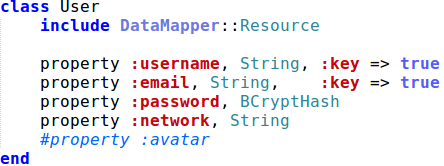
\includegraphics[width=7cm]{./images/chefmanagement-model-user.png}
		\caption{Modelo usuario} \label{fig:chefmanagement-model-user}
	\end{figure}

	\item \textbf{Recetas (Recipe):} Este modelo contiene información sobre la receta creada por un determinado usuario. Establece la relación con la clase Usuario, del que depende de uno a muchos (1:M) y con las clases ingredientes y recetas base, cuya relación es en ambos casos de 1:M. Tiene muchos campos, de los que cabe destacar: \emph{name}, nombre de la receta y clave primaria; \emph{nration}, campo requerido y que indica el número de platos, y \emph{username} que es el autor de la receta. 	Sus relaciones son: una receta puede tener varios ingredientes (clase Ingredients) o varias recetas base (clase Recipe2).

	\begin{figure}[H]
		\centering
		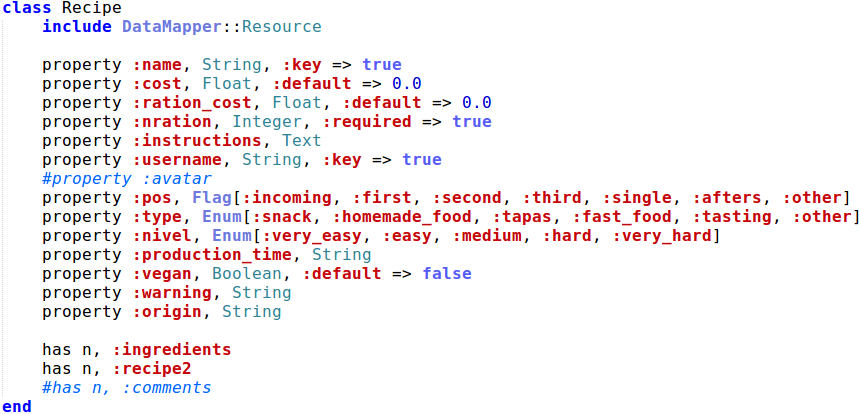
\includegraphics[width=12cm]{./images/chefmanagement-model-recipe.png}
		\caption{Modelo receta} \label{fig:chefmanagement-model-recipe}
	\end{figure}

	\item \textbf{Ingredientes (Ingredient):} Se trata de los ingredientes para cada receta. Por lo tanto depende de la clase receta con una relación de 1:M. Sus campos más importantes son su \emph{id} (clave primaria), \emph{name} que es el nombre del ingrediente y \emph{cost} que corresponde a su coste, siendo estos dos último campos requeridos.

	\begin{figure}[H]
		\centering
		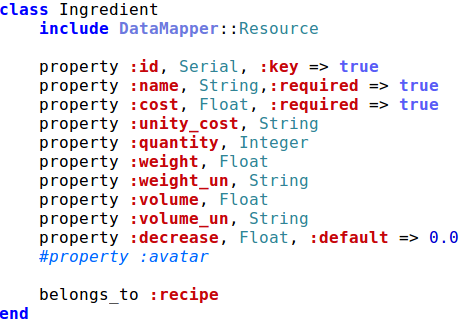
\includegraphics[width=8cm]{./images/chefmanagement-model-ingredient.png}
		\caption{Modelo ingrediente} \label{fig:chefmanagement-model-inredient}
	\end{figure}

	\item \textbf{Recetas base (Recipe2):} Esta clase es una extensión de recipe, que sirve para identificar las recetas usadas como ingredientes en otras, esto es una receta base. Su relación con la clase receta se presenta de 1:M.

	\begin{figure}[H]
		\centering
		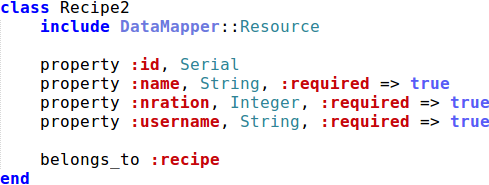
\includegraphics[width=9cm]{./images/chefmanagement-model-recipe2.png}
		\caption{Recetas base} \label{fig:chefmanagement-model-recipe2}
	\end{figure}

\end{itemize}

Puede ver con detalle el código fuente del modelo de la aplicación en \href{https://github.com/alu0100207385/ChefManagement/blob/master/app/models/model.rb}{model.rb}.


%%%%%%%%%%%%%%%%%%%%%%%%%%%%%%%%%%%%%%%%%%%%%%%%%%%%%%%%%%%%%%%%%%%%%%%%%%%%%%%
\newpage{\pagestyle{empty}\cleardoublepage}
\thispagestyle{empty}

\chapter{Gestión de la configuración}
\label{chapter:tres}

%%%%%%%%%%%%%%%%%%%%%%%%%%%%%%%%%%%%%%%%%%%%%%%%%%%%%%%%%%%%%%%%%%%%%%%%%%%%%%%
% Chapter 3: Gestión de la configuración
%%%%%%%%%%%%%%%%%%%%%%%%%%%%%%%%%%%%%%%%%%%%%%%%%%%%%%%%%%%%%%%%%%%%%%%%%%%%%%%

\section{PaaS}\label{cap.3.1}

En el capítulo de introducción~\ref{chapter:intro} se explicó los cambios en la elección del entorno de producción, así como su estudio. En este capítulo se explicará los dos entornos de producción escogidos, cómo funcionan y se configuran. \\

Antes de empezar debe quedar claro los modelos de servicios que ofrecen las nubes. Las empresas ofertan distintos servicios y prestaciones, de los cuales destacan:
\begin{itemize}
	\item \textbf{SaaS:} Software como servicio. Se trata de cualquier servicio basado en la web. En este tipo de servicios accedemos normalmente a través del navegador sin atender al software. Todo el desarrollo, mantenimiento, actualizaciones, copias de seguridad es responsabilidad del proveedor. Son ejemplos conocidos \emph{Google docs, Hotmail o Dropbox.}
	\item \textbf{PaaS:} Plataforma como servicio, es una encapsulación del entorno de desarrollo y un conjunto de módulos con el fin de proporcionar una funcionalidad que se traduce como servicio. En este modelo de servicio al usuario se le ofrece la plataforma de desarrollo y las herramientas de programación por lo que puede desarrollar aplicaciones propias y controlar la aplicación, pero no controla la infraestructura. Por ejemplo, \emph{Heroku, Google App Engine o Windows Azure}. 
	\item \textbf{IaaS:} Infraestructura como servicio. Tendremos más control que con PaaS, lo que implica la gestión de la infraestructura. Es un medio de entregar almacenamiento básico y capacidades de cómputo como servicios estandarizados en la red. Servidores, sistemas de almacenamiento, conexiones, enrutadores, y otros sistemas se concentran para manejar tipos específicos de cargas de trabajo. Algunos ejemplos son: \emph{Amazon Web Services, Google Cloud Storage y VMware}. 
\end{itemize}

Para esta aplicación, trabajaremos con el modelo PaaS. Normalmente, para interactuar con la PaaS elegida, el proveedor proporciona una herramienta. Esta cambia en función de la nube elegida, pero su funcionamiento y opciones son similares: descargar la aplicación de un determinado repositorio y hacerla correr en la nube a modo de producción. Además ofrecen distintos servicios o módulos, normalmente de pago. En Heroku se conoce como \emph{dynos} y en OpenShift se llama \emph{cartridge}. Éstos pueden ser la base de datos con la que interactuará la aplicación, mejoras en el equipo servidor (nube de producción) como mayor capacidad de disco, memoria RAM, CPU, sistema dedicado, incluso aumentar el ancho de banda para atender más peticiones.

\begin{figure}[H]
	\centering
	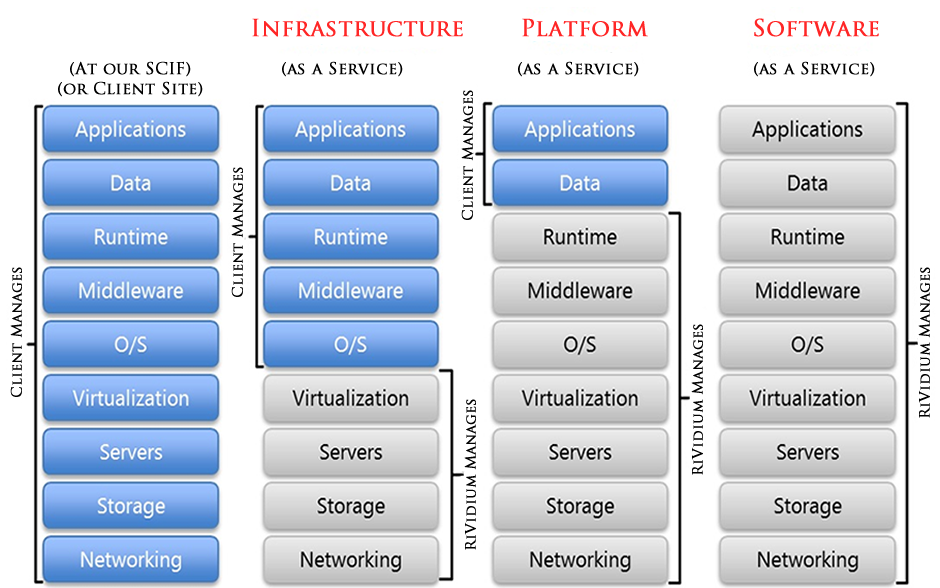
\includegraphics[width=12cm]{./images/cloud-models.png}
	\caption{Modelos de nubes} \label{fig:cloud-models}
\end{figure}

\vspace*{0.2in}
\section{Heroku}\label{cap.3.2}

Se trata de una plataforma de aplicaciones cloud que permite construir y desplegar aplicaciones web. Soporta distintos lenguajes y frameworks. Para poder usar esta plataforma lo primero es registrarse y acceder a la misma. Desde la pantallas de \emph{dashboard} podremos gestionar las aplicaciones o bien mediante los comandos de su herramienta (\href{https://devcenter.heroku.com/start}{\emph{Heroku Toolbelt}}). Existen tres formas de configurar nuestra aplicación en Heroku.
\begin{itemize}
	\item El \textbf{dashboard}: Desde esta pantalla seleccionamos la app deseada y encontramos un menu con una serie de opciones que nos permiten gestionar la aplicación en la nube: añadir add-ons, activar \emph{dynos}, seleccionar repositorio, información como métricas y actividad del servidor, permiso de acceso a la app y la configuración propia de la app (variables, dominio, etc.).
	\item Mediante \textbf{Heroku Toolbelt}: Este comando (\$ heroku COMMAND) tiene múltiples opciones que permiten interactuar con la consola desde consola. Subir app, configurar la bbdd y variables, comprobar logs del servidor, etc. En resumen, las opciones que nos proporciona el \emph{dashboard} en el navegador, pero desde consola. Ejecute \$ heroku -h para acceder a la ayuda y opciones.
	\item A través de \textbf{archivos de configración}: Esta opción afecta más a la configuración de la propia aplicación. Aquí podemos crear variables, base de datos y otros, sin embargo, no se gestionan los dynos o add-ons pero sí usarlos o interactuar con ellos si están creados.
\end{itemize}

Para integrar la base de datos en producción podemos hacerlo de dos formas:
\begin{itemize}
	\item Utilizar la herramienta con el comando: \$ heroku addons:create heroku-postgresql.
	\item O bien, desde el \emph{Dashboard} $\rightarrow$ Settings $\rightarrow$ Config Variables.
\end{itemize}

Para visualizar la configuración general usaremos el comando \$ heroku config. Con esta varible ya podemos crear el adaptador para la aplicación. En este proyecto se trabaja con \href{http://datamapper.org/}{DataMapper} para el manejo y creación de la bbdd. De forma general, su configuración es: \\

\begin{figure}[H]
	\centering
	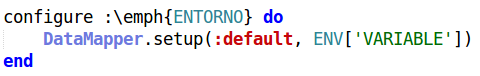
\includegraphics[width=8cm]{./images/env01.png}
	\caption{Configuración de la BBDD con DataMapper} \label{fig:env01}
\end{figure}
 
 donde:
 \begin{itemize}
	 \item \emph{ENTORNO}: es el entorno para el que se está configurando: desarrollo, test o producción.
	\item default: la configuración por defecto. Podemos establecer un archivo de configuración por defecto. Las nubes de producción tienen el suyo, aunque a veces hay que adaptarlo a nuestras necesidades o crear nuestra propia configuración.
	\item ENV['VARIABLE']: corresponde a una variable que guarda la ruta a la base de datos. También puede ponerse la ruta directamente pero no es recomendable.
\end{itemize}

En nuestro caso sería: \\

\begin{figure}[H]
	\centering
	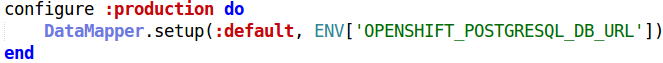
\includegraphics[width=9cm]{./images/env02.png}
	\caption{Configuración de la BBDD para Chefmanagement} \label{fig:env02}
\end{figure}

Debido a que en OpenShift no puede modificarse el nombre de las variables, la renombramos en Heroku de igual forma para utilizar una única varible de configuración que es válida para ambos entornos de producción a la vez. Cada servidor contendrá este nombre de variable con un adaptador distinto.


\vspace*{0.2in}
\section{OpenShift}\label{cap.3.3}
Es otra PaaS similar a la anterior montada en Linux Red Hat. Permite desarrollar rápidamente, hosting y la escalabilidad de aplicaciones en entornos de la nube. Al contrario que Heroku, en la versión \emph{free} permite crear hasta tres aplicaciones (y la primera cinco), sin embargo, aunque Heroku solo permite postgresql en esta versión, OpenShift permite escoger entre MongoDB, MySQL y PostgreSQL. Para \textbf{ChefManagement}, hemos tenido que adaptarnos al cuello de botella de Heroku en cuanto bbdd y trabajaremos con postgres en ambas plataformas. \\

Aunque OpenShift no dispone de tantas opciones de configuración en su \emph{dashboard} si que permite añadir \emph{cartridges} inclusos creados por nosotros mismos. Por ejemplo, un \href{https://github.com/openshift-cartridges/jruby-cartridge}{cartucho} para hacer funcionar Jruby en OpenShift. \\

En cuanto a la \href{https://developers.openshift.com/en/managing-client-tools.html}{herramienta del cliente} permite la gestión con la nube de igual forma que con la herramienta de Heroku. Sin embargo, en esta nube, no se puede añadir ni modificar variables. La nube almacena la configuración por defecto en caso de que la proporcionada no sea válida. En todo caso habría que usar su herramienta o archivos de configuración. \\

Los archivos de configuración son muy útles si no queremos usar las variables por defecto que proporciona la nube. Hay dos formas de editar estos archivos, mediante la herramienta cliente o bien editando manualmente estos \href{https://blog.openshift.com/netsource-partners-shows-the-benefits-of-custom-environment-variables-on-openshift/}{archivos de configuración}. \\

Para configurar el adaptador de la base de datos en OpenShift podemos \href{https://developers.openshift.com/en/managing-environment-variables.html}{crear la variable} de la siguiente forma:
\begin{center}
	\$ rhc env set VARIABLE=VALUE --a App\_Name
\end{center}

Por defecto en esta nube esta información esta almacenada en la variable OPENSHIFT\_POSTGRESQL\_DB\_URL. Podemos acceder a la nube y consultar todas las variables mediante ssh:
\begin{center}
\$ rhc ssh APLICACION
\end{center}

Para ver la lista de variables creadas escribimos en consola \$ rhc env-list --a chefmanagement, y para ver todas las variables de entorno nos conectamos por ssh y usamos el comando \emph{env}.


%%%%%%%%%%%%%%%%%%%%%%%%%%%%%%%%%%%%%%%%%%%%%%%%%%%%%%%%%%%%%%%%%%%%%%%%%%%%%%%
\newpage{\pagestyle{empty}\cleardoublepage}
\thispagestyle{empty}

\chapter{Metodología de desarrollo}
\label{chapter:cuatro}

%%%%%%%%%%%%%%%%%%%%%%%%%%%%%%%%%%%%%%%%%%%%%%%%%%%%%%%%%%%%%%%%%%%%%%%%%%%%%%%
% Chapter 4: Metodología de desarrollo
%%%%%%%%%%%%%%%%%%%%%%%%%%%%%%%%%%%%%%%%%%%%%%%%%%%%%%%%%%%%%%%%%%%%%%%%%%%%%%%

%++++++++++++++++++++++++++++++++++++++++++++++++++++++++++++++++++++++++++++++
En el capítulo~\ref{chapter:intro} se exlpicó la metodología ágil. En este capítulo repasaremos esta metodología usando como ejemplo el desarrollo de \textbf{Chefmanagement} y también el modelo-vista-controlador y su estructura.

\vspace*{0.2in}
\section{Metodología ágil}\label{cap.4.1}

Se había comentado anteriormente el uso de la metodología ágil, esto es debido a la naturaleza del proyecto: se trata de crear una aplicación en un período determinado y cuyas características no están claras, lo cual se debe a que los requisistos no están definidos, no existe un cliente con una necesidad, en este caso se trata de experimentar. Dentro de este tipo de metodologías, se ha usado \emph{Scrum} para obtener resultados rápidamente y donde los requisistos pueden cambiar en cada iteración. La necesidad de innovar y la flexibilidad responden bien con esta metodología. \\

Hay que tener en cuenta, que debido a las circunstancias de este proyecto (no hay un equipo de desarrollo ni un cliente propiamente dicho) se ha adaptado \emph{Scrum} a las necesidades, sin embargo, esta metodología se ha realizado de forma estricta en reuniones con el tutor y en la elaboración de la aplicación. A continucación se explica de forma general una iteración durante el desarrollo de esta aplicación:
\begin{itemize}
	\item \textbf{Planificación:} Cómo me iba a organizar el trabajo durante esa semana. Planificar tiempo a cada una de las siguientes etapas. Corresponde a las reuniones semanales con el tutor y programar los nuevos requisitos en función de los resultados obtenidos.
	\item \textbf{Análisis de requisitos:} Cada vez que se proponía una idea ésta era analizada con el fin de comprobar su viabilidad en la aplicación. Se trata del estudio de campo e investigaciones específicas según la tarea planificada.
	\item \textbf{Diseño:} Cada vez que se desee agregar una funcionalidad al programa se debe estudiar el cambio en el diseño de la misma, de forma que optimice su usabilidad. El diseño también hace referencia a la forma en la que se va a crear los distintos modelos de la base de datos y sus relaciones. Crear la estructura del proyecto de forma que sea escalable.
	\item \textbf{Codificación:} Parte del tiempo en el que se desarrollaba código. Durante el estudio de campo esta etapa se destino a crear programas sencillos de prueba.
	\item \textbf{Revisión:} Comprobar la aplicación hasta el punto actual. Tanto las características nuevas como las anteriores. También se incluyen las pruebas de código.
	\item \textbf{Documentación:} Durante el tiempo de vida del proyecto se ha ido elaborando un diario, en él se guarda la información de los resultados obtenidos semanalmente y expuestos durante las reuniones: lo qué se ha averiguado, lo qué se ha conseguido, los problemas encontrados y las soluciones propuestas.
\end{itemize}

\vspace*{0.2in}
\section{Estructura de la app}\label{cap.4.2}
La aplicación ha sido diseñada y desarrollada de acuerdo con el framework de \href{http://www.sinatrarb.com/}{Sinatra} cuya arquitectura software se base en el MVC. Por un lado define componentes para la representación de la información, y por otro la interacción del usuario. La filosofía de este modelo es la reutilización de código y la separación de conceptos, características que buscan facilitar la tarea de desarrollo de aplicaciones y su posterior mantenimiento. \\

\begin{figure}[H]
	\centering
	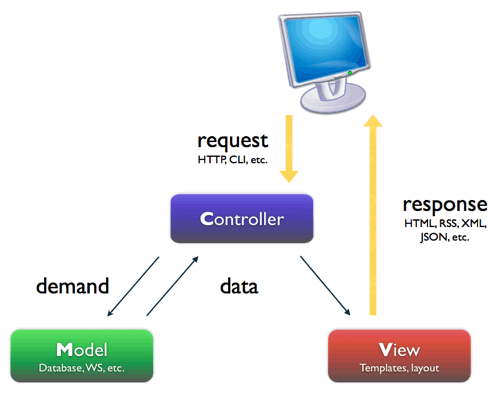
\includegraphics[width=10cm]{./images/mvc.png}
	\caption{Modelo-Vista-Controlador} \label{fig:MVC}
\end{figure}

Durante la etapa de análisis y estudio de campo se empezó diseñando en \href{http://rubyonrails.org/}{Ruby on Rails}, otro framework en lenguaje Ruby, sin embargo, uno de los requisitos era que la aplicación sea soportada bajo JRuby. Durante las pruebas muchas de gemas utilizadas en Rails presentaban problemas de incompatibilidad por lo que había que bajarlas de versión, y esto a su vez con otras y la aplicación. Es el caso de la \emph{gema ActiveRecord}. 

\begin{figure}[H]
	\centering
	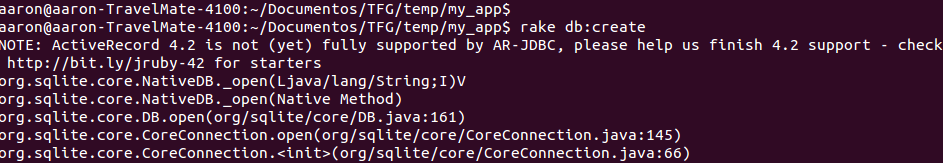
\includegraphics[width=12cm]{./images/activerecord-message.png}
	\caption{ActiveRecord 4.2 no está soportado completamente por JRuby} \label{fig:AvtiveRecord-no-supported}
\end{figure}

La idea de la compatibilidad con JRuby se considera importante para este proyecto no solo para ampliar el soporte de la aplicación, también en futuros módulos como el desarrollo en plataformas móviles o tablets con \href{http://ruboto.org/}{Ruboto}, cuyas apps pueden ser desarrolladas usando JRuby, MRI o Rubinius. \\

Por esta razón, y la libertad en diseño de la aplicación que proporciona Sinatra frente a Rails, así como su sencilla puesta en marcha, se optó finalmente por este framwork para el desarrollo de Chefmanagament. La estructura que se diseñó es la siguiente (también puede verse en el \href{https://github.com/alu0100207385/ChefManagement}{repositorio}):

\begin{itemize}
	\item \textbf{app}: la codificación modelo-vista-controlador se encuentra aquí. Contiene el modelo, el contolador y las vistas de la aplicación, así como funciones auxiliares (helpers) y los tests.
		\begin{itemize}
			\item config.yml: contiene los tokens e identificadores para las distintas APIs y correo usado por la aplicación.
			\item controllers: gestiona la aplicación en función de las peticiones del usuario e interactúa con el modelo y las vistas (salida al usuario).
			\item helpers: son funciones auxiliares definidas específicamente para esta aplicación. Cabe destacar el uso de la gema \href{https://github.com/mikel/mail}{Mail} para la gestión de acceso, registro y notificaciones de la aplicación.
			\item models: diseño de la base de datos. Más información en la sección~\ref{cap.2.6}
			\item tests: la definición y declaración de las pruebas. Además de comprobar las funciones y métodos creados, se ha utilizado la herramienta \href{http://www.seleniumhq.org/}{Selenium} para interactuar con la propia aplicación y pornerla a prueba. Puede ver los resultados en \href{https://travis-ci.org/alu0100207385/ChefManagement?branch=testing}{Travis}.
			\item views: su función es interactuar con el usuario, es el resultado de las acciones del usuario con la aplicación, en un formato que éste pueda entener, como páginas webs.
		\end{itemize}
	\item \textbf{public}:
		\begin{itemize}
			\item css: el estilo de las vistas.
			\item js: los archivos javascripts que controlan las entrada de datos e informan al usuario.
			\item uploads: está destinada a almacenar los archivos importados y exportados de las listas de recetas de cada usuario.
			\item resources: carpeta para almacenar recursos como imágenes, etc.
			\item otros: otras carpetas de apis usadas en la aplicación.
		\end{itemize}
	\item .travis.yml: archivo de configuración para realizar las pruebas de la aplicación en un servidor remoto. Se trata de un modelo de integración continua. Se configuró de forma que se realizaran las pruebas en distintos navegadores: Firefox (por defecto) y Chrome.
	\item Gemfile: contiene las gemas configuradas en los distintos entornos (desarrollo, producción y tests) para que la aplicación pueda funcionar.
	\item Procfile: archivo de configuración de inicio del servidor en las nubes de producción.
	\item Rakefile: contiene las distintas tareas y opciones que se pueden realizar. 
	\item config.ru: inicia la aplicación bajo \emph{rackup}.
\end{itemize}


%%%%%%%%%%%%%%%%%%%%%%%%%%%%%%%%%%%%%%%%%%%%%%%%%%%%%%%%%%%%%%%%%%%%%%%%%%%%%%%
\newpage{\pagestyle{empty}\cleardoublepage}
\thispagestyle{empty}

\chapter{Conclusiones y trabajos futuros}
\label{chapter:conclusiones}

%%%%%%%%%%%%%%%%%%%%%%%%%%%%%%%%%%%%%%%%%%%%%%%%%%%%%%%%%%%%%%%%%%%%%%%%%%%%%
% Chapter 5: Conclusiones y Trabajos Futuros 
%%%%%%%%%%%%%%%%%%%%%%%%%%%%%%%%%%%%%%%%%%%%%%%%%%%%%%%%%%%%%%%%%%%%%%%%%%%%%%%

%++++++++++++++++++++++++++++++++++++++++++++++++++++++++++++++++++++++++++++++
Conclusiones aqui

\begin{center}
	\rule{80mm}{0.3mm}\\
\end{center}

A continuación se propone mejoras para incluir en módulos de futuras versiones de la aplicación:

\begin{itemize}
\item Integrar APIs de precios de productos de proveedores (Mercadona, Alcampo, etc). Esto permite un precio real y actualizado de la receta. Aunque no está integrada en la aplicación se propone usar el \href{http://www.opendatacanarias.es/datos/dataset/mercatenerife-precios-de-productos-hortofruticolas-de-tenerife}{listado de productos} (en formato json) de \textbf{Mercatenerife}.

\item Actualizar y mejorar el diseño con temas personalizables.
\item Incluir en el modelo información sobre el plato (kcal, proteínas, hidratos, grasas, etc.).
\item Añadir a la funcionalidad \emph{Calculadora} evaluar los \textbf{costos de menús}.
\item Desarrollo en dispositivos smatphones y tablets, aprovechando la compatibilidad con JRuby se propone desarrollar en \textbf{Ruboto}.

\item La aplicación puede diversificarse atendiendo a su mercado: \textbf{profesional} (negocios de restauración) o enfoque de \textbf{red social}.
	\item Para el mercado de red social se propone:
		\begin{itemize}
			\item \textbf{Sistema de puntuación}: comprar recetas o conseguir a través de las puntuaciones que consigas compartiendo tus recetas.
			\item \textbf{Otras características de red social}: compartir recetas, marcar como favoritos, comentarios, etc.
			\item \textbf{Estadísticas}: platos-puntos, usuarios-recetas, platos-precio, etc.
		\end{itemize}
	\item Para el mercado de negocio:
		\begin{itemize}
			\item \textbf{Buscar} un determinado ingrediente en un determinado momento. Ver el precio actual.
			\item \textbf{Comprar} al proveedor a través de la aplicación.
		\end{itemize}

\end{itemize}


%%%%%%%%%%%%%%%%%%%%%%%%%%%%%%%%%%%%%%%%%%%%%%%%%%%%%%%%%%%%%%%%%%%%%%%%%%%%%%%
\newpage{\pagestyle{empty}\cleardoublepage}
\thispagestyle{empty}
 
\chapter{Summary and Conclusions} 
\label{chapter:summary}

%%%%%%%%%%%%%%%%%%%%%%%%%%%%%%%%%%%%%%%%%%%%%%%%%%%%%%%%%%%%%%%%%%%%%%%%%%%%%
% Chapter 6: Summary and Conlusions
%%%%%%%%%%%%%%%%%%%%%%%%%%%%%%%%%%%%%%%%%%%%%%%%%%%%%%%%%%%%%%%%%%%%%%%%%%%%%%%

%++++++++++++++++++++++++++++++++++++++++++++++++++++++++++++++++++++++++++++++

Over the course of this document we have seen different aspects associated with the development of \textbf{Chefmanagement}, using agile methodology. It has been used the knowledge gained during academic education, this includes research and analysis and actual practice in projects and companies. \\

Thanks to the experience gained in enterprise practices I have given importance to market research, this has led me to interviews with various restaurants and suppliers to know their needs on the application. Also, the idea of innovation in this type of application includes a field study of them. \\

We must also take into account the investigation of production clouds, tests and analyse which is best suited to this project needs. \\

In short, this project includes protocols and methodologies such as Scrum (Agile methodology), using frameworks based on MVC, TDD (local and on remote servers) use of repositories and cloud programming. \\

It has been introduced a new PaaS (OpenShift) and a new application has been developed in order to continue evolving, trying to design a scalable and even exportable to other architectures.

%%%%%%%%%%%%%%%%%%%%%%%%%%%%%%%%%%%%%%%%%%%%%%%%%%%%%%%%%%%%%%%%%%%%%%%%%%%%%%%
\newpage{\pagestyle{empty}\cleardoublepage}
\thispagestyle{empty}

\chapter{Presupuesto}
\label{chapter:presupuesto}

%%%%%%%%%%%%%%%%%%%%%%%%%%%%%%%%%%%%%%%%%%%%%%%%%%%%%%%%%%%%%%%%%%%%%%%%%%%%%
% Chapter 7: Presupuesto
%%%%%%%%%%%%%%%%%%%%%%%%%%%%%%%%%%%%%%%%%%%%%%%%%%%%%%%%%%%%%%%%%%%%%%%%%%%%%%%

%++++++++++++++++++++++++++++++++++++++++++++++++++++++++++++++++++++++++++++++

En este capítulo abordaremos el caso comercial de puesta en marcha de la aplicación propuesta creando un presupuesto para su desarrollo. Vamos a partir del supuesto siguiendo los datos de la asignatura de TFG de un trabajo realizado de 300 h. y un precio de 12 \euro/h. \\

\begin{document}

Como gastos en producción se propone dos entornos a elegir uno:

\begin{itemize}

\item \textbf{Opción 1: Heroku}
\begin{center}
    \begin{tabular}{| l | l | r | p{5cm} |}
    \hline
    Servicio & Base & Subtotal & Comentario \\ \hline
    Horas trabajadas & 300 & 3600 & 300 h x 12 \euro/h \\ \hline
    Heroku & 67.34 (\euro/mes) & 808.08 & Se calcula el precio para un año. Se ha elegido la opción estándar.\\ \hline
    Confiración & 60 & 60 & Gastos para preparar y configurar el entorno de producción. \\ \hline 
    Otros gastos & 60 & 180 & Gastos destinados a entrevistas. En este caso 3. \\ \hline 
    Mantenimiento & 300 (\euro/año) & 0 & Este servicio es gratis el primer año. \\ \hline
    \textbf{TOTAL} &  & 4648.08 \euro &  \\
    \hline
    \end{tabular}
\end{center}

Estos precios son variables en función del tiempo y las prestaciones contratadas, puede calcularse de forma online en \href{https://www.heroku.com/pricing}{Heroku}, aunque el precio se calcula en dólares americanos. 

\item \textbf{Opción 2: OpenShift}
\begin{center}
    \begin{tabular}{| l | l | r | p{5cm} |}
    \hline
    Servicio & Base & Subtotal & Comentario \\ \hline
    Horas trabajadas & 300 & 3600 & 300 h x 12 \euro/h \\ \hline
    OpenShift & 15 (\euro/mes) & 180 & Se calcula el precio para un año. Se ha elegido la opción estándar base.\\ \hline
    Confiración & 60 & 60 & Gastos para preparar y configurar el entorno de producción. \\ \hline 
    Otros gastos & 60 & 180 & Gastos destinados a entrevistas. En este caso 3. \\ \hline 
    Mantenimiento & 300 (\euro/año) & 0 & Este servicio es gratis el primer año. \\ \hline
    \textbf{TOTAL} &  & 4020 \euro & \\
    \hline
    \end{tabular}
\end{center}

En el caso de esta PaaS podemos consultar sus \href{https://www.openshift.com/products/pricing/plan-comparison}{precios} según las necesidades. El precio está calculado para el plan \emph{Silver}.

\end{itemize}

%%%%%%%%%%%%%%%%%%%%%%%%%%%%%%%%%%%%%%%%%%%%%%%%%%%%%%%%%%%%%%%%%%%%%%%%%%%%%%%

%%%%%%%%%%%%%%%%%%%%%%%%%%%%%%%%%%%%%%%%%%%%%%%%%%%%%%%%%%%%%%%%%%%%%%%%%%%%%%%
%\newpage{\pagestyle{empty}\cleardoublepage}
%\thispagestyle{empty}
%\begin{appendix}

%\chapter{Título del Apéndice 1}
%\label{appendix:1}
%\input{apendice1.tex}

%\chapter{Título del Apéndice 2}
%\label{appendix:2}
%\input{apendice2.tex}

%\end{appendix}

%%%%%%%%%%%%%%%%%%%%%%%%%%%%%%%%%%%%%%%%%%%%%%%%%%%%%%%%%%%%%%%%%%%%%%%%%%%%%%%
\newpage{\pagestyle{empty}\cleardoublepage}
\thispagestyle{empty}

\chapter{Glosario}
\label{chapter:glossary}

%%%%%%%%%%%%%%%%%%%%%%%%%%%%%%%%%%%%%%%%%%%%%%%%%%%%%%%%%%%%%%%%%%%%%%%%%%%%%
% Chapter: Glosario
%%%%%%%%%%%%%%%%%%%%%%%%%%%%%%%%%%%%%%%%%%%%%%%%%%%%%%%%%%%%%%%%%%%%%%%%%%%%%%%

nube - cloud \\
SaaS \\
escandallo \\
Jruby \\
Sinatra \\
TDD \\
PaaS \\
GAE \\
Scrum \\
MVC \\
CRUD \\

%%%%%%%%%%%%%%%%%%%%%%%%%%%%%%%%%%%%%%%%%%%%%%%%%%%%%%%%%%%%%%%%%%%%%%%%%%%%%%%

%%%%%%%%%%%%%%%%%%%%%%%%%%%%%%%%%%%%%%%%%%%%%%%%%%%%%%%%%%%%%%%%%%%%%%%%%%%%%%%
\addcontentsline{toc}{chapter}{Bibliografía}
\bibliographystyle{plain}

\bibliography{memtfg}
% \nocite comentado, para que solo salga la biblio citada
%\nocite{*}

%%%%%%%%%%%%%%%%%%%%%%%%%%%%%%%%%%%%%%%%%%%%%%%%%%%%%%%%%%%%%%%%%%%%%%%%%%%%%%%

\end{document}
